\begin{figure*}
\centering
\scalebox{0.8}{
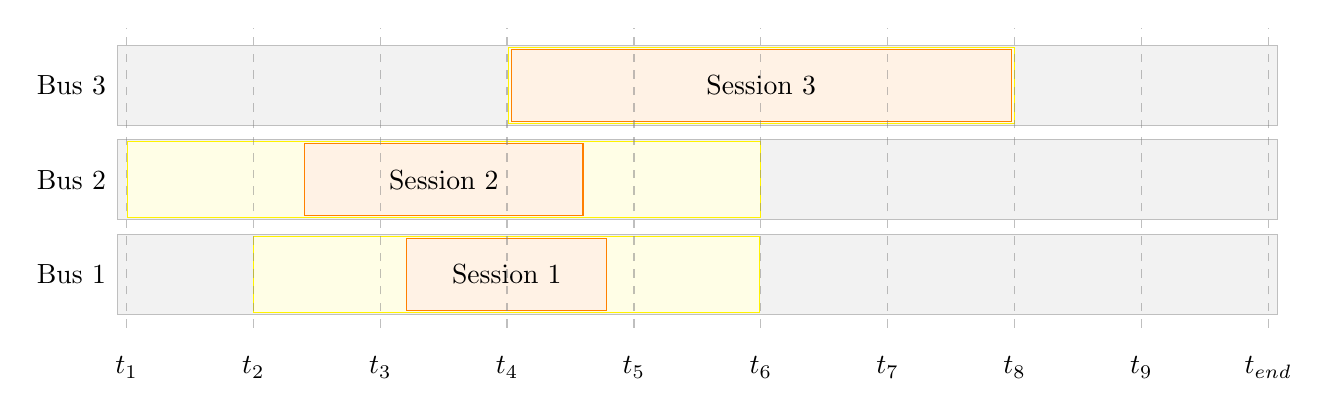
\begin{tikzpicture}
	\node[rectangle, draw=gray!50, fill=gray!10, minimum width=5.8in, minimum height=0.4in](bus1Box) at (7.75,0.8){};
	\node(bus1BoxLabel) at (-0.2, 0.8){Bus 1}; 
	\node[rectangle, draw=yellow!100, fill=yellow!10, minimum width=2.53in, minimum height=0.38in](charge11) at (5.33, 0.8){};
	\node[rectangle, draw=orange!100, fill=orange!10, minimum width=1in, minimum height=0.36in](charge111) at (5.33, 0.8){Session 1};

	\node[rectangle, draw=gray!50, fill=gray!10, minimum width=5.8in, minimum height=0.4in](bus2Box) at (7.75,2){};
	\node(bus1BoxLabel) at (-0.2, 2.0){Bus 2};
	\node[rectangle, draw=yellow!100, fill=yellow!10, minimum width=3.1625in, minimum height=0.38in](charge11) at (4.53, 2){};
	\node[rectangle, draw=orange!100, fill=orange!10, minimum width=1.3915in, minimum height=0.36in](charge111) at (4.53, 2){Session 2};
	
	\node[rectangle, draw=gray!50, fill=gray!10, minimum width=5.8in, minimum height=0.4in](bus3Box) at (7.75,3.2){};
	\node(bus1BoxLabel) at (-0.2, 3.2){Bus 3}; 
	\node[rectangle, draw=yellow!100, fill=yellow!10, minimum width=2.53in, minimum height=0.38in](charge11) at (8.56, 3.2){};
	\node[rectangle, draw=orange!100, fill=orange!10, minimum width=2.50in, minimum height=0.36in](charge111) at (8.56, 3.2){Session 3};


	\foreach \curLab/\preLab[count=\c, evaluate=\c as \pos using {0.5 + (\c - 1)*14.5/9}] in {t_1/t_1, t_2/t_1, t_3/t_2, t_4/t_3, t_5/t_4, t_6/t_7, t_7/t_6, t_8/t_7, t_9/t_8, t_{end}/t_9}
		{
			\node[label=below:$\curLab$](b\c) at (\pos, 0){};
			\node(t) at (\pos, 3.8){};
			\draw[dashed, line width=0.5pt, black!50, opacity=0.5] (b\c.north) -- (t.north); 
		}
		\path (b9.south) -- node[midway, below=0.1in]{$\hdots$}(b10.south); 
\end{tikzpicture}}
\caption{Demonstrates how results from $p_4$ can be reexpressed in terms of continuous variables} 
\label{fig:refactorExample}
\end{figure*}


